\scanpage{72}
% archive sheet number: 71

constructible $\underline{Q}_p$-sheaves on $k$ to the category $\mathrm{Fcriso}(k)$. For an object \deleted{$E$}$(E,F_E)$ of the latter, the following conditions are equivalent\inserted{\unsure{\deleted{x}(|\deleted{(}x}if $k$ perfect\unsure{\deleted{x})|\deleted{)}x}}\handwritten{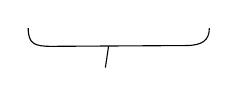
\begin{tikzpicture}[x=1cm,y=1cm,baseline=0cm]\draw[thin] (0,.2)..controls (0,0) and (.08,-.03)..(.3,-.03)--(2,-.02)..controls (2.2,-.02) and (2.3,.04)..(2.3,.2);\draw[thin] (1.02,-.03)--(.98,-.3);\end{tikzpicture}}: a) $(E,F_E)$ belongs to the essential image of the preceding functor; b) there exists a lattice $M\subset E$ stable under $F_E$ \deleted{over} \uline{\unsure{\deleted{l}a|\deleted{e}a}nd} under $F_E^{-1}$ (i.e. such that $F_E$ induces an \uline{automorphism} of $M$); c) the family of i\unsure{\handwritten{t}|\deleted{e}\handwritten{t}|\deleted{o}\handwritten{t}|\deleted{a}\handwritten{t}}erates $F^{\unsure{n|m}}$, $n\quad\underline{Z}$, is bounded ; d) $E$ and $\overset{\handwritten{\vee}}{E}$ are effective.

The F-isocrystals in question are called ``trivial'' or ``\uline{of slope zero}''. One thus finds an \uline{epimorphism of gerbes}
\figure{\[
\underline{G}(k)\handwritten{\longrightarrow}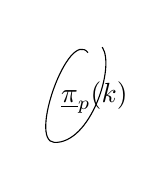
\begin{tikzpicture}[baseline=(gerbe.base)]
\node[inner sep=1pt] (gerbe) {$\handwritten{\underline{\pi}_{p}}(k)$};
\handwritten{\draw[thin] (-0.08,0.57) .. controls (-0.33,0.88) and (-0.84,-0.55) .. (-0.51,-0.57) .. controls (-0.05,-0.59) and (0.27,0.39) .. (0.10,0.64);}
\end{tikzpicture}\ ,
\]}
\margin{\handwritten{$\Pi$\par capital?}}
where $\handwritten{\underline{\unsure{\Pi|\pi}}}_p(k)$ is the gerbe over $\underline{Q}_p$ \deleted{of continuous representations} associated with the Tannakian category of constructible $\underline{Q}_p$-sheaves, equivalent \deleted{to the algebraic envelope} (once an algebraic closure $\bar{k}$ of $k$ has been chosen) to the trivial gerbe defined by the algebraic \deleted{of the} $p$-adic envelope of the profinite group $\handwritten{\pi}=\operatorname{Gal}(\handwritten{\bar{k}}/k)$. Taking account of the augmentation homomorphism of \unsure{\deleted{T}G|\deleted{G}T}ate, one even finds a homomorphism
\[
\underline{G}(k)\handwritten{\longrightarrow\underline{\pi}}_p(k)\ \mathrm{x}\ \handwritten{[}\underline{G}_m\handwritten{]}_{\underline{Q}_p}
\]
where $\handwritten{[}\underline{G}_m\handwritten{]}$ is the trivial gerbe defined by $\underline{G}_m$ . One easily checks that this is again an epimorphism (i.e. that the functor
\[
(V_i)_{\handwritten{i}}\handwritten{\longmapsto\sum}V_i\otimes_{\underline{\unsure{\not Q|\mathbb{Q}}}_p}\underline{Q}_p(i)
\]
going from the category of \deleted{\unsure{sh|ch}} \inserted{\handwritten{grad\unsure{e|e}d}} constructible $\underline{Q}_p$-sheaves \handwritten{\begin{tikzpicture}[x=1cm,y=1cm,baseline=0cm]\draw[thin] (0,-.35)..controls (.12,-.15) and (-.05,.1)..(.4,.25)..controls (1.2,.4) and (2.25,.7)..(2.5,.92)..controls (2.65,1.1) and (2.55,1.22)..(2.4,1.2);\end{tikzpicture}} on $k$ to $\mathrm{Fcriso}(k)$ is fully faithful). The F-isocrystals of the preceding form could be called the F-isocrystals \uline{of level zero} .

\handwritten{6.} Let us now consider a homomor\unsure{\^{p}|\deleted{ô}p|\deleted{p}ô}\unsure{\.{h}|\deleted{i}h|\deleted{h}i}ism of fields\textsubscript{\unsure{x|\deleted{x}}}
\[
k\handwritten{\longrightarrow}k'\ ,
\]
whence a homomorphism of Tannakian categories over $\underline{Q}_p$
\[
\mathrm{Fcriso}(k)\handwritten{\longrightarrow}\mathrm{Fcriso}(\deleted{\unsure{i|t|k}}\handwritten{k}')\ ,
\]
and a homomorphism of Tannakian gerbes over $\underline{Q}_p$ in the opposite direction

\mspage{71}
